\section{Group -- Plant-Condenser Flow Control}\label{group-plant-condenser-flow-control}

The connector list described earlier determines how the branches of a particular loop will be hooked together. These connections can be classified either as a separation of a single stream into several outlet streams (splitter) or the merging of several streams into a single outlet stream (mixer). Due to the limitation per branch of a single splitter and a single mixer, the connector list can only have two pieces of equipment as a maximum. The names defined for either/both the splitter or/and the mixer refer then to ``component'' definitions as described below.

\subsection{Connector:Splitter, Connector:Mixer}\label{connectorsplitter-connectormixer}

The format of both the \textbf{\hyperref[connectorsplitter]{Connector:Splitter}} and \textbf{\hyperref[connectormixer]{Connector:Mixer}} statements is similar. Both begin with an identifying name followed by the branch name of the ``single side'' of the component. In the case of the splitter, this is the inlet since the inlet stream is broken into several outlet streams. In the case of the mixer, this is the outlet since several streams are mixed together to form a single outlet. The remaining list of up to 50 names is simply the branch names of the outlet legs in the case of the splitter and inlet legs in the case of the mixer. No control logic is assume in these components---a determination of how much air to split in which direction using the splitter must be defined by other components.

\subsection{Connector:Splitter}\label{connectorsplitter}

\subsubsection{Inputs}\label{inputs-034}

\paragraph{Field: Name}\label{field-name-033}

This alpha field contains the identifying name for the Splitter.

\paragraph{Field: Inlet Branch Name}\label{field-inlet-branch-name}

This alpha field contains the identifying name for the Splitter Inlet Branch.

\paragraph{Field: Outlet Branch \textless{}x\textgreater{} Name}\label{field-outlet-branch-x-name}

This alpha field contains the identifying names for the Splitter Outlet Branches and you enter as many outlet branches as needed.

\subsection{Connector:Mixer}\label{connectormixer}

\subsubsection{Inputs}\label{inputs-1-031}

\paragraph{Field: Name}\label{field-name-1-030}

This alpha field contains the identifying name for the Mixer.

\paragraph{Field: Outlet Branch Name}\label{field-outlet-branch-name}

This alpha field contains the identifying name for the Mixer Outlet Branch.

\paragraph{Field: Inlet Branch \textless{}x\textgreater{} Name}\label{field-inlet-branch-x-name}

This alpha field contains the identifying names for the Mixer Inlet Branches and you enter as many inlet branch names as needed..

An example of these statements in an IDF is:

\begin{lstlisting}

Connector:Splitter,
               CW Loop Splitter,
               CW Pump Branch,
               Little Chiller Branch,
               Big Chiller Branch,
               Purchased Cooling Branch,
               Supply Bypass Branch;
  Connector:Mixer,
               CW Loop Mixer,
               Cooling Supply Outlet,
               Little Chiller Branch,
               Big Chiller Branch,
               Purchased Cooling Branch,
               Supply Bypass Branch;
\end{lstlisting}

\subsection{TemperingValve}\label{temperingvalve}

This object is used for special cases where plant flow control is needed to make efficient use of thermal storage. In certain solar hot water and heat recovery situations, a thermal storage tank may become warmer than is necessary or allowable for safe use of the hot water. Although real installations of a tempering, or anti-scald valve, would more commonly mix a new stream of mains water with the hot water to achieve a desired outlet temperature, this is difficult to model directly within EnergyPlus because plant loops need to be closed circuits. For many installations where the water entering the splitter is directly from the mains, such as make up water entering a water heater tank, the modeling provided with this object should be thermodynamically equivalent.

The TemperingValve object models a temperature-controlled diversion valve. It models a valve on a bypass pipe that can open to divert flow around one or more plant components. It can only be used on one of two branches between a Splitter and a Mixer. The figure below shows the use of the tempering valve with a Water Heater:Mixed component on ``Stream 2.''~ The tempering valve acts to divert flow through the branch it is on in order to adjust the temperature at the outlet of the mixer. If the temperature at Stream 2 Source Node is warmer than the setpoint and the inlet flow is cooler than the setpoint, then a controller determines how much flow should bypass the storage tank to achieve the desired setpoint.

\begin{figure}[hbtp] % fig 89
\centering
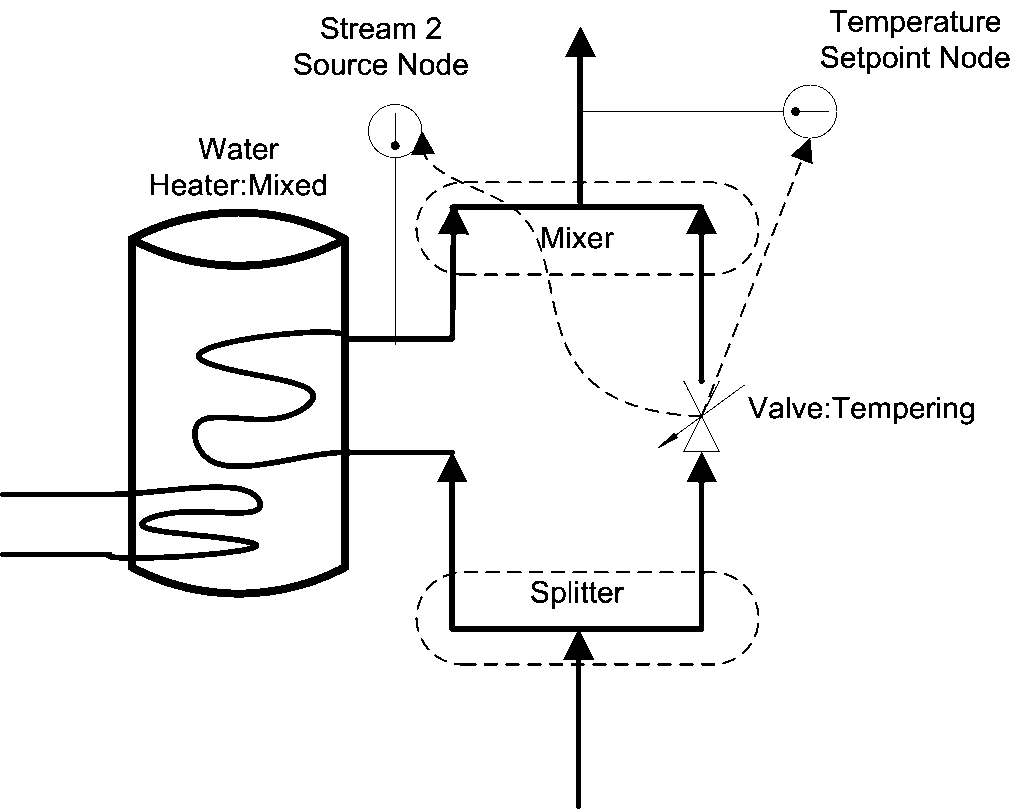
\includegraphics[width=0.9\textwidth, height=0.9\textheight, keepaspectratio=true]{media/image208.png}
\caption{Tempering Valve Schematic \protect \label{fig:tempering-valve-schematic}}
\end{figure}

The TemperingValve is an \textbf{Active} component and the other path should have only \textbf{Passive} components. Passive components are ones that can make a flow request but will passively accept whatever flow is provided by the loop. Active components specifically set the flow. When using the TemperingValve, only two paths can be used in the splitter/mixer; bypasses are not allowed. No other \hyperref[connectorsplitter]{Connector:Splitter} and \hyperref[connectormixer]{Connector:Mixer} pair can be used on the supply side of the plant loop.

\subsubsection{Inputs}\label{inputs-2-029}

\paragraph{Field: Name}\label{field-name-2-028}

This field should contain an unique name for each TemperingValve object

\paragraph{Field: Inlet Node Name}\label{field-inlet-node-name-003}

This field should contain the name of node which is the inlet for the valve.

\paragraph{Field: Outlet Node Name}\label{field-outlet-node-name-004}

This field should contain the name of node which is the outlet for the valve

\paragraph{Field: Stream 2 Source Node Name}\label{field-stream-2-source-node-name}

This field should contain the name of node that is the inlet to the Mixer object for the second stream containing the component whose flow is being diverted.

\paragraph{Field: Temperature Setpoint Node Name}\label{field-temperature-setpoint-node-name-000}

This field should contain the name of a node that has a temperature setpoint assigned to it. A separate set point manager object is needed to provide a set point on the node listed here.

\paragraph{Field: Pump Outlet Node Name}\label{field-pump-outlet-node-name}

This field should contain the name of the node that is the outlet for the pump that is on the same plant loop. This node is used to sense the total flow rate.

This object is demonstrated in the example file called SolarCollectorFlatPlateWater.idf. An example of this object is:

\begin{lstlisting}

TemperingValve,
          DHW Anti-Scald Diverter,
          DHW Anti-Scald Inlet Node, ! Inlet Node Name
          DHW Anti-Scald Outlet Node, ! Outlet Node Name
          SHW Storage Tank Use Outlet Node, ! Stream 2 Source Node Name
          DHW Instantaneous Boost Outlet Node, ! Temperature Setpoint Node Name
          DHW Use Side Pump Outlet;  ! pump outlet node
\end{lstlisting}

\subsubsection{Outputs}\label{outputs-023}

Use output variables for System Nodes for flow and temperature results.